\documentclass[10pt,letterpaper]{article}
\usepackage[margin=0.78in]{geometry}
\usepackage{fontspec}
\usepackage{microtype}
\usepackage{amsmath,amssymb}
\usepackage{booktabs,tabularx,array,longtable}
\usepackage{graphicx}
\usepackage{xcolor}
\usepackage[font=small,labelfont=bf]{caption}
\usepackage{enumitem}
\usepackage[colorlinks=true,linkcolor=teal!70!black,citecolor=teal!70!black,urlcolor=blue!60!black]{hyperref}
\setlength{\parskip}{0.42em}
\setlength{\parindent}{0pt}
\sloppy
\emergencystretch=1.8em
\definecolor{hdrnavy}{HTML}{0F172A}

\title{\textbf{\Large Multi-Scale Normal-Tissue Injury Tiers and Symmetric Enrichment Reconcile Cancer--Testis Antigen Discovery Across Human, Dog, and Mouse and Map Actionable TCR-T, CAR-T, ADC, and Radioligand Modalities}}
\author{\textbf{PIRL-UNC Collaborative Group}\\ \small Computational Oncology \& Immunogenomics, University of North Carolina at Chapel Hill \\ \footnotesize \texttt{https://github.com/pirl-unc/oncoref} $\cdot$ Policy \texttt{oncoref.target-selection.2026-11-27.1}}
\date{November 2026 $\cdot$ Preprint}

\begin{document}
\maketitle
\begin{abstract}
\noindent \textbf{Background:} Cancer--testis antigens (\texttt{CTAs}) and oncofetal proteins anchor affinity-enhanced T-cell receptor therapies (\texttt{TCR-T}), bispecific \texttt{ImmTACs}, vaccines, and emerging surface-directed \texttt{CAR-T}, antibody--drug conjugate (\texttt{ADC}), and radioligand (\texttt{RLT}) modalities. Yet across \textbf{149} published studies nominating \textbf{2,233} human protein groups, gene lists diverge sharply because legacy screens pool incompatible expression units, dilute rare neuroendocrine or sensory cells in bulk organ biopsies, conflate biological germline expression with patient-specific organ expendability, and transfer human labels onto dog and mouse models by symbol orthology.\\[0.3em]
\textbf{Methods:} We developed a species-invariant four-stage screening architecture (\texttt{OncoRef}, policy \texttt{2026-11-27.1}) that (i) collapses identical translations into protein-equivalence groups (\texttt{PEGs}) while screening all isoforms for $\ge 95\%$ 9-mer \texttt{Unsafe} containment; (ii) evaluates every healthy somatic and activated-immune dataset in its native measurement unit (\texttt{TPM}, \texttt{nTPM}, \texttt{nCPM}, donor-resolved droplet \texttt{UMI}, \texttt{IHC}, or plex-bleed-corrected \texttt{TMT-ppm}) across four clinical organ-injury tiers (\texttt{Vital}, \texttt{Protected}, \texttt{Manageable}, \texttt{Disposable}); (iii) enforces symmetric $\ge 10 \times H_0$ \emph{in vivo} enrichment over $H_0 = \max(N, D, 1\text{ TPM})$ in tumors (\texttt{CA}) and reproductive/embryonic compartments (\texttt{RA}), defining $\text{CTA} = \text{CA} \cap \text{RA}$ while segregating pure \emph{in vitro} cell lines; and (iv) couples candidates to \texttt{HostContext} organ protection, 0/1-mismatch \texttt{PeptideIndex} self-subtraction, and UniProtKB extracellular-domain modality mapping.\\[0.3em]
\textbf{Results:} Across \textbf{19,893} human (\texttt{GRCh38}), \textbf{20,082} domestic dog (\texttt{CanFam3.1}), and \textbf{21,433} laboratory mouse (\texttt{GRCm39}) \texttt{PEGs} (8/8 pillars active natively per species), OncoRef identifies \textbf{322 human}, \textbf{118 canine}, and \textbf{8 murine} \emph{in vivo} \texttt{CTAs} (96.6\%, 96.6\%, and 75.0\% ectopic). Segregating pure cell lines unmasks host \texttt{NK} \texttt{TIL} granzymes (\texttt{Gzmd--g}) in syngeneic grafts, and only \textbf{15/433} mammalian \texttt{CTA} ortholog families qualify as \texttt{CTAs} in $\ge 2$ species due to primate \texttt{CT-X}/\texttt{ZGA} expansion. In humans, \textbf{78.8\% (1,760/2,233)} of published nominations are \texttt{Unsafe} while rules uncover \textbf{77} unnominated \texttt{CTAs}; \texttt{CTA-M} (222) outnumbers \texttt{CTA-F} (12) by \textbf{18.5:1} alongside \textbf{48} adult-absent \texttt{CTA-P} antigens (270 female-safe vs.\ 60 male-safe \texttt{CTAs}). Primary-literature review of all \textbf{66} baseline \texttt{CA only} proteins adjudicates \textbf{7} occult adult human \texttt{Vital}/\texttt{Protected} niche proteins (\texttt{GALP}, \texttt{BHLHE23}, \texttt{IL36B}, \texttt{ZACN}, \texttt{HES3}, \texttt{OCSTAMP}, \texttt{PROKR1}) to \texttt{Unsafe} and \textbf{6} sensory/C-cell/paralog holds to \texttt{Other:Review}, resolving all \textbf{53} retained \texttt{CA only} proteins into five somatic-silent biological classes. Against \textbf{16} clinical \texttt{TCR-T}/\texttt{ImmTAC} trials, OncoRef flags \textbf{6/6 (100\%)} severe specificity toxicities as \texttt{Unsafe} while retaining \textbf{5/5 (100\%)} safe potent \texttt{CTAs}. Subcellular topology mapping shows \textbf{84.0\% (315/375)} of human \texttt{CAs} are intracellular (\texttt{TCR-T}/\texttt{ImmTAC}) and \textbf{9.6\% (36)} secreted, while \textbf{24 (6.4\%)} expose plasma-membrane ectodomains---including \textbf{19} with $\ge 50\text{ aa}$ mature ectodomains (\texttt{BTN1A1}, \texttt{ERVV-1/2}, \texttt{CIROP}, \texttt{CRIPTO3}, \texttt{ADAM2}, \texttt{ADAM18}, \texttt{FMR1NB}, \texttt{CT83}, \texttt{ZP4}, \texttt{IZUMO1R}, \texttt{LYPD4}, \texttt{PKDREJ}) actionable for \texttt{CAR-T}, \texttt{ADC}, and \texttt{RLT} without the somatic liabilities carried by \textbf{24/24 (100\%)} of conventional clinical surface benchmarks.
\end{abstract}

\section{Introduction}
Affinity-enhanced T-cell receptor therapies (\texttt{TCR-T}) and soluble TCR--anti-CD3 bispecific engagers (\texttt{ImmTACs}) recognize intracellularly processed peptides bound to major histocompatibility complex (\texttt{pMHC}) molecules at single-digit copy numbers per cell, producing durable clinical responses against \texttt{MAGEA4} (\emph{afamitresgene autoleucel}), \texttt{NY-ESO-1}/\texttt{CTAG2} (\emph{letetresgene autoleucel}), and \texttt{PRAME} (\texttt{IMA203}, \emph{brenetafusp}) [1--5]. That same sensitivity triggered lethal necrotizing leukoencephalopathy via rare brain \texttt{MAGEA12} cross-recognition (\texttt{NCT01273181}) [6], lethal cardiogenic shock within 4--5 days via striated-muscle \texttt{Titin} (\texttt{TTN}) mimotope cross-reactivity (\texttt{NCT01350401}) [7], dose-limiting hemorrhagic colitis against colonic \texttt{CEACAM5} [8], and uveitis plus cochlear hair-cell ototoxicity against melanocytic \texttt{MLANA} and \texttt{PMEL} [9].

Across \textbf{149} published CTA, oncofetal, zygotic-genome-activation (\texttt{ZGA}), and placental studies nominating \textbf{2,233} human protein groups [10--14], four methodological failure modes recur: (1) cross-scale pooling of incompatible units (\texttt{TPM}, \texttt{nTPM}, \texttt{CP10K}, microarray) and bulk-organ dilution of $<1\%$ vital neuroendocrine or sensory cell populations by $50\text{--}1,000\times$; (2) pre-analytical sequencing artifacts including multiplex flowcell index hopping, plate pipetting splash, nuclear pre-mRNA cis-readthrough (\texttt{GAB3 $\rightarrow$ CTAG2}), and tumor genomic DNA (\texttt{gDNA}) background; (3) conflation of biological germline expression with patient-conditional organ expendability; and (4) naive gene-symbol projection across human, companion-dog, and murine genomes. Here we present the unified \texttt{OncoRef} framework resolving all four challenges and mapping every retained candidate onto intracellular \texttt{pMHC} versus surface \texttt{CAR-T}/\texttt{ADC}/\texttt{RLT} therapeutic modalities.

\section{Conceptual Architecture: Native Scales, Injury Tiers, and Set Algebra}
\begin{figure}[htbp]
\centering
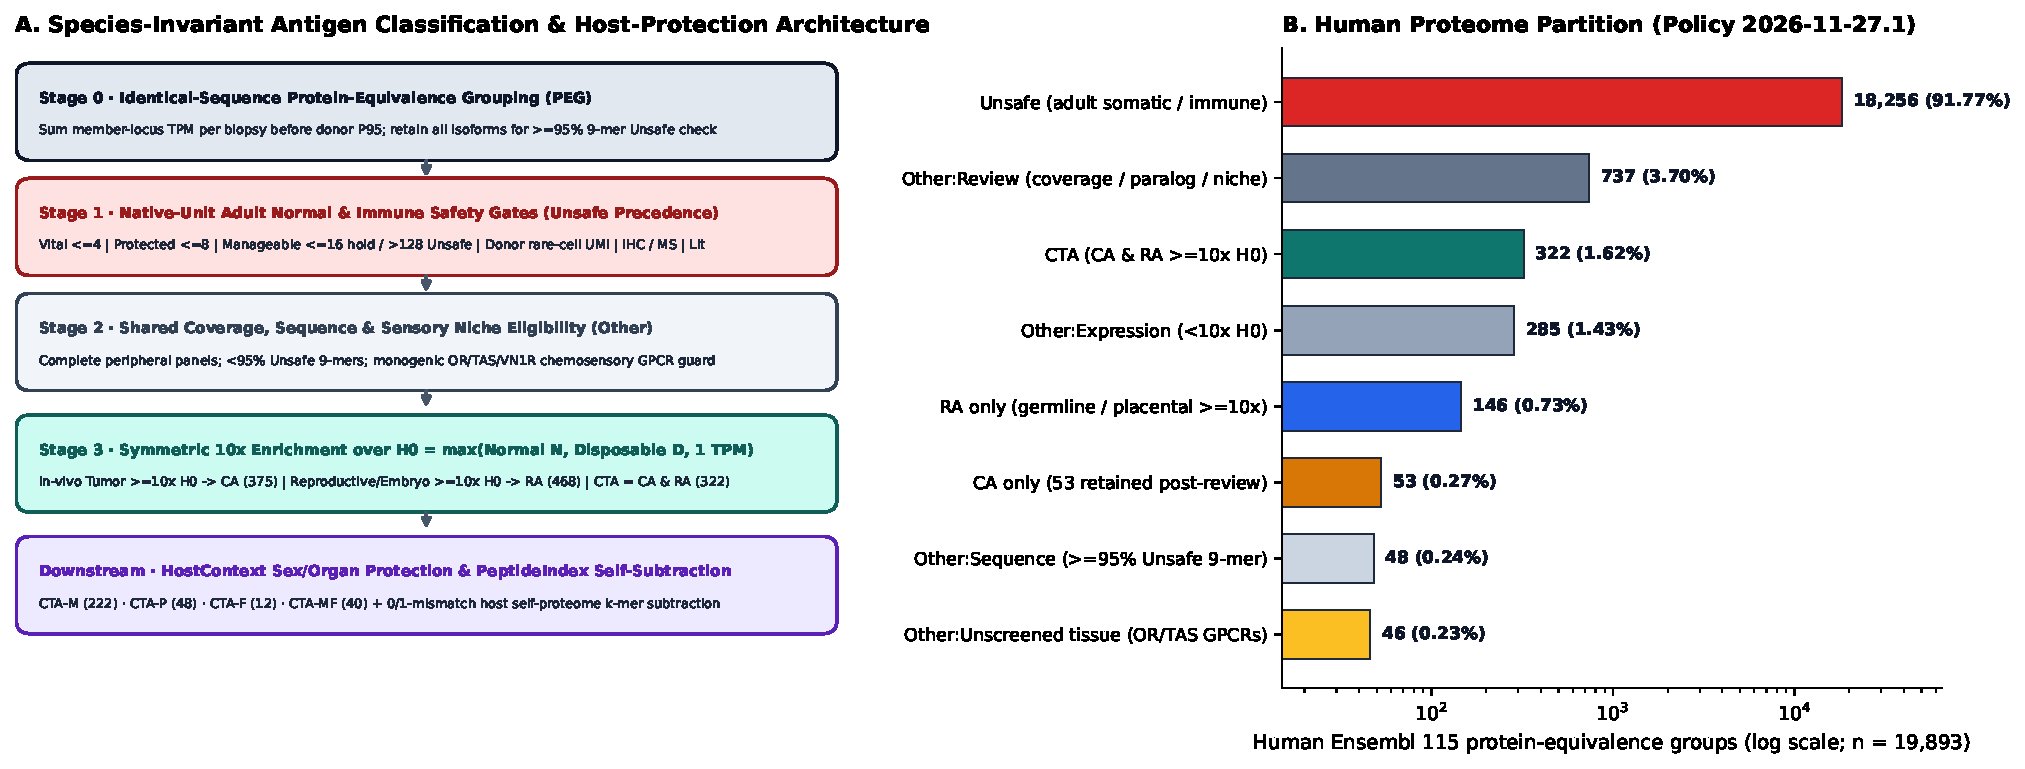
\includegraphics[width=\textwidth]{figures/fig1-conceptual-architecture-and-attrition.pdf}
\caption{\textbf{Conceptual pipeline architecture and human proteome attrition.} \textbf{(A)} Species-invariant Stages 0--3 decoupled from downstream \texttt{HostContext} organ protection and \texttt{PeptideIndex} self-proteome subtraction. \textbf{(B)} Partition of all 19,893 human Ensembl 115 protein-equivalence groups (20,099 coding loci).}
\label{fig:arch}
\end{figure}

\textbf{Stage 0 (Protein-equivalence grouping and pre-analytical QC).} Primary-assembly coding loci with identical canonical/MANE representative translations collapse into a single \texttt{PEG}, summing complete member-locus abundance within each library before summarizing across donors while retaining all splice isoforms (245,535 human, 45,036 canine, and 66,037 murine records) for $\ge 95\%$ 9-mer \texttt{Unsafe} containment. Holistic \texttt{NNLS} deconvolution across 18,637 GTEx v11 libraries (52 shards, 946 donors: 311 XX, 635 XY) quarantines 2 foreign-organ swaps and strips 201 SM-plate splash events, 100,287 index-hopping pairs, 225 same-donor carryovers, and 16,058 boundary admixtures. Libraries exceeding $2.5\%$ olfactory receptors $\ge 5\text{ TPM}$ fail \texttt{gDNA} QC, admixed \texttt{TGCT} biopsies cannot act as sole tumor witnesses, and purely nuclear pre-mRNA cis-spillover with zero cytoplasmic/bulk RNA and negative IHC is recorded as \texttt{nuclear\_only} caution.

\textbf{Stage 1 (Four clinical adult tissue-injury tiers without unit conversion).} Every non-reproductive structure and sorted immune lineage maps to a cited injury tier: \textbf{\texttt{Vital}} ($\le 4.0$ native bulk units: CNS, retina, inner-ear hair cells, DRG, heart, lung, liver, kidney, adrenal, pancreas, endothelium, HSCs, platelets), \textbf{\texttt{Protected}} ($\le 8.0$: GI/urinary/esophageal/corneal/skin epithelia, smooth/skeletal muscle, peripheral nerve, thyroid follicular parenchyma, pituitary, mature T/NK/monocyte/macrophage/neutrophil subsets), \textbf{\texttt{Manageable}} (hold $>16.0$, \texttt{Unsafe} $>128.0$: B cells, gallbladder, spleen, thyroid parafollicular C-cells), and \textbf{\texttt{Disposable}} ($D \le 32.0$: hair follicle, non-ocular skin melanocytes, tonsil, appendix, minor salivary gland, and separately tracked involuted adult thymus). Bulk RNA donor P95, single-cell cluster \texttt{nCPM}, donor-resolved droplet \texttt{UMI} ($\ge 10$ cells and $\ge 1\%$ multi-UMI cells replicated across $\ge 2$ studies/$\ge 3$ donors, or $\ge 5\%$ single-study; $2\times$ in \texttt{Protected}), protein staining/\texttt{TMT-ppm}, and curated adult human literature act in their native scales with strict \texttt{Unsafe} precedence.

\textbf{Stages 2--3 (Eligibility guards, symmetric $10\times H_0$ enrichment, and \texttt{HostContext}).} Surviving proteins require complete peripheral coverage (\texttt{Other:Review}), $<95\%$ \texttt{Unsafe} 9-mer overlap (\texttt{Other:Sequence}), and a screened home niche---holding all unvalidated monogenic chemosensory GPCRs (\texttt{OR*}, \texttt{TAAR*}, \texttt{TAS1R/2R*}, \texttt{VN1R*}) out of \texttt{CA}/\texttt{CTA}. Against $H_0 = \max(N, D, 1\text{ TPM})$, \emph{in vivo} tumor enrichment $T_{\max} \ge 10 H_0$ defines \texttt{CA}, reproductive or supported embryo-lineage enrichment $R_{\text{supp}} \ge 10 H_0$ defines \texttt{RA}, and $\text{CTA} = \text{CA} \cap \text{RA}$ (pure cell lines populate \texttt{cell\_line\_max\_tpm} only). Downstream \texttt{HostContext} protection yields four mutually exclusive classes (\texttt{CTA-M}, \texttt{CTA-P}, \texttt{CTA-F}, \texttt{CTA-MF}), followed by exact and 1-mismatch \texttt{PeptideIndex} self-proteome subtraction.

\section{Multi-Species Inventory and Parameterization: Human, Dog, and Mouse}
\begin{table}[htbp]
\centering
\scriptsize
\setlength{\tabcolsep}{3.5pt}
\caption{Genome-wide screening parameterization and category partition across human, domestic dog, and laboratory mouse (\texttt{oncoref.target-selection.2026-11-27.1}).}
\label{tab:species}
\begin{tabularx}{\textwidth}{l l r c l X r r r r}
\toprule
\textbf{Species} & \textbf{Reference} & \textbf{PEGs (Loci)} & \textbf{Pillars} & \textbf{Tumor / Line Scope} & \textbf{CTA (Sex)} & \textbf{CA only} & \textbf{RA only} & \textbf{Other} & \textbf{Unsafe} \\
\midrule
Human (9606) & Ensembl 115 & 19,893 (20,099) & 8/8 & 135 cohorts & 322 (222M/48P/12F/40MF) & 53 & 146 & 1,116 & 18,256 \\
Dog (9615) & Ensembl 98 & 20,082 (20,199) & 8/8 & 19 coh (935) + 12 CL & 118 (100M/7P/1F/10MF) & 127 & 313 & 2,201 & 17,323 \\
Mouse (10090) & Ensembl 115 & 21,433 (21,760) & 8/8 & 14 coh (57) + 9 CL & 8 (5M/2P/0F/1MF) & 30 & 303 & 2,514 & 18,578 \\
\bottomrule
\end{tabularx}
\end{table}
\begin{figure}[htbp]
\centering
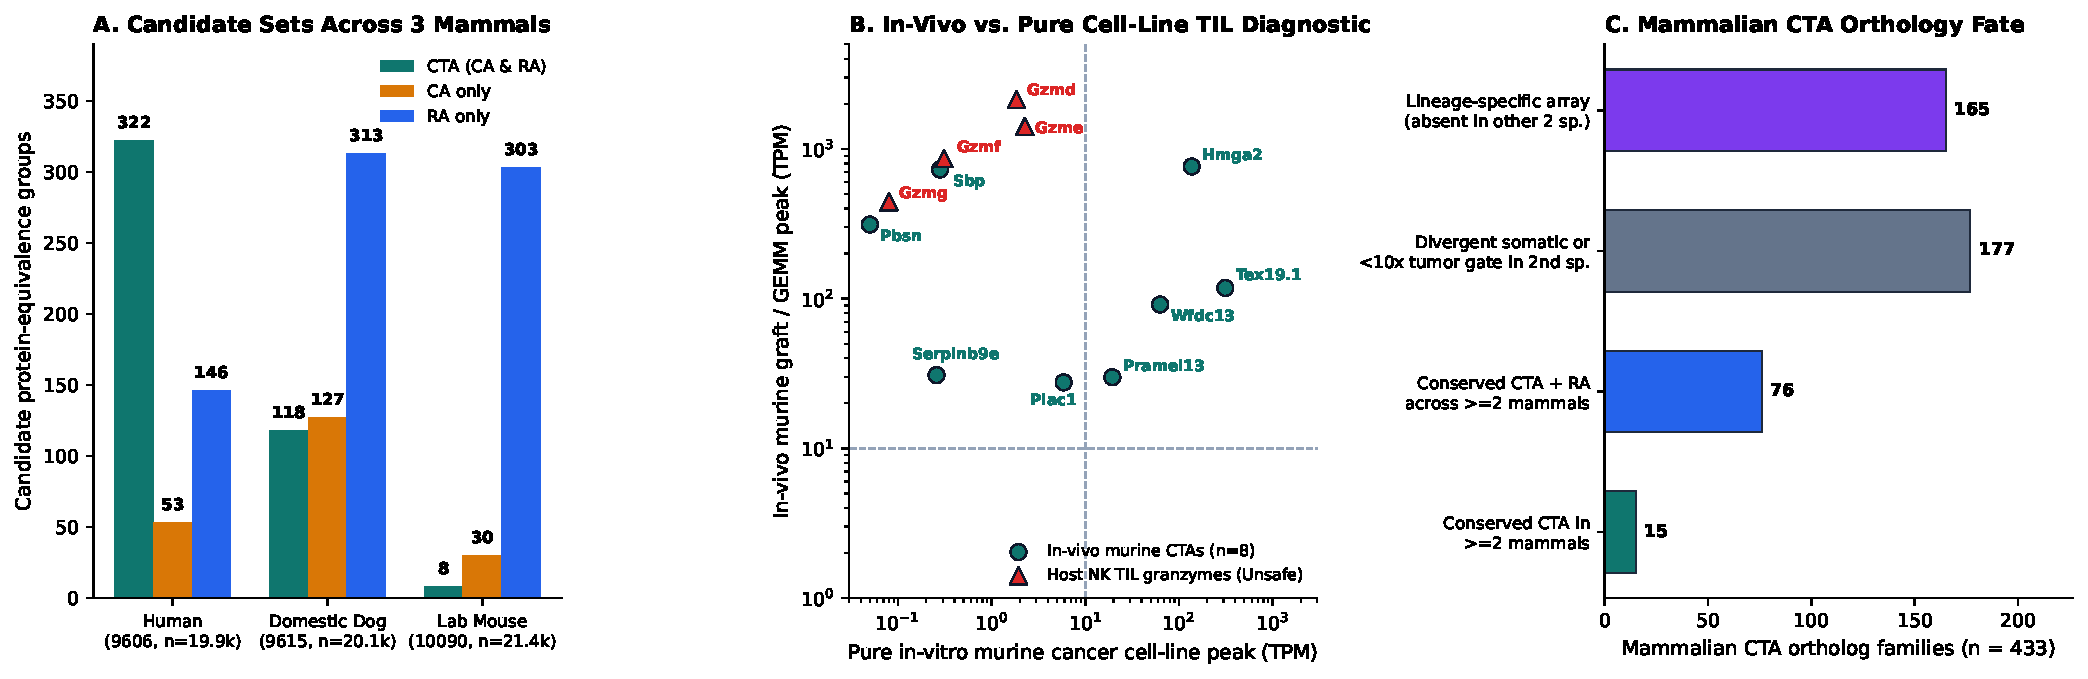
\includegraphics[width=\textwidth]{figures/fig2-multispecies-parameterization-and-orthology.pdf}
\caption{\textbf{Multi-species parameterization, cell-line TIL diagnostic, and mammalian CTA orthology.} \textbf{(A)} Candidate sets across human, dog, and mouse (8/8 pillars active per species). \textbf{(B)} Murine \emph{in vivo} graft/GEMM TPM vs.\ pure cultured tumor cell-line TPM separating intrinsic CTAs from host NK TIL granzymes (\texttt{Gzmd--g}). \textbf{(C)} Fate of 433 mammalian CTA ortholog families.}
\label{fig:species}
\end{figure}

Evaluating all eight screening pillars natively in \emph{Homo sapiens} (\texttt{GRCh38}), outbred companion \emph{Canis lupus familiaris} (\texttt{CanFam3.1}; lacking seminal vesicles and appendix, screened across Bgee 15.2, 300-sample \texttt{GSE219045}, 64 mammary biopsies \texttt{GSE119810}, 7-dog healthy PBMC 10x \texttt{GSE225599}, 38-tissue plex-bleed-corrected \texttt{TMT-ppm} proteomics, and 19 spontaneous patient cohorts), and \emph{Mus musculus} (\texttt{GRCm39}; possessing coagulating gland, lacking tonsil/appendix and adult male mammary ducts, screened across Bgee 15.2, \texttt{GSE219045}, ImmGen + activated NK/Treg/BMDM RNA, Tabula Muris 10x, MGI GXD TS28, and 14 \emph{in vivo} cohorts) yields \textbf{322}, \textbf{118}, and \textbf{8} \emph{in vivo} \texttt{CTAs} (Table~\ref{tab:species}, Fig.~\ref{fig:species}). Segregating pure \emph{in vitro} cancer cell lines unmasks cytolytic granzymes \texttt{Gzmd--g} ($443\text{--}2,138\text{ TPM}$ in \emph{in vivo} \texttt{MC38}/\texttt{CT26}/\texttt{B16F10} grafts vs.\ $0.08\text{--}2.26\text{ TPM}$ in pure cultured tumor cells) as infiltrating host \texttt{NK} \texttt{TIL} transcripts, while only \textbf{15/433} mammalian \texttt{CTA} ortholog families qualify as \texttt{CTAs} in $\ge 2$ species because primate \texttt{CT-X}/\texttt{ZGA} arrays (\texttt{NY-ESO-1}, \texttt{GAGE}, \texttt{SPANX}, \texttt{XAGE}, \texttt{VCX/Y}, \texttt{DUX4}) evolved after boreoeutherian divergence.

\section{Human Proteome Deep Dive and the 66-Protein \texttt{CA only} Review}
\begin{figure}[htbp]
\centering
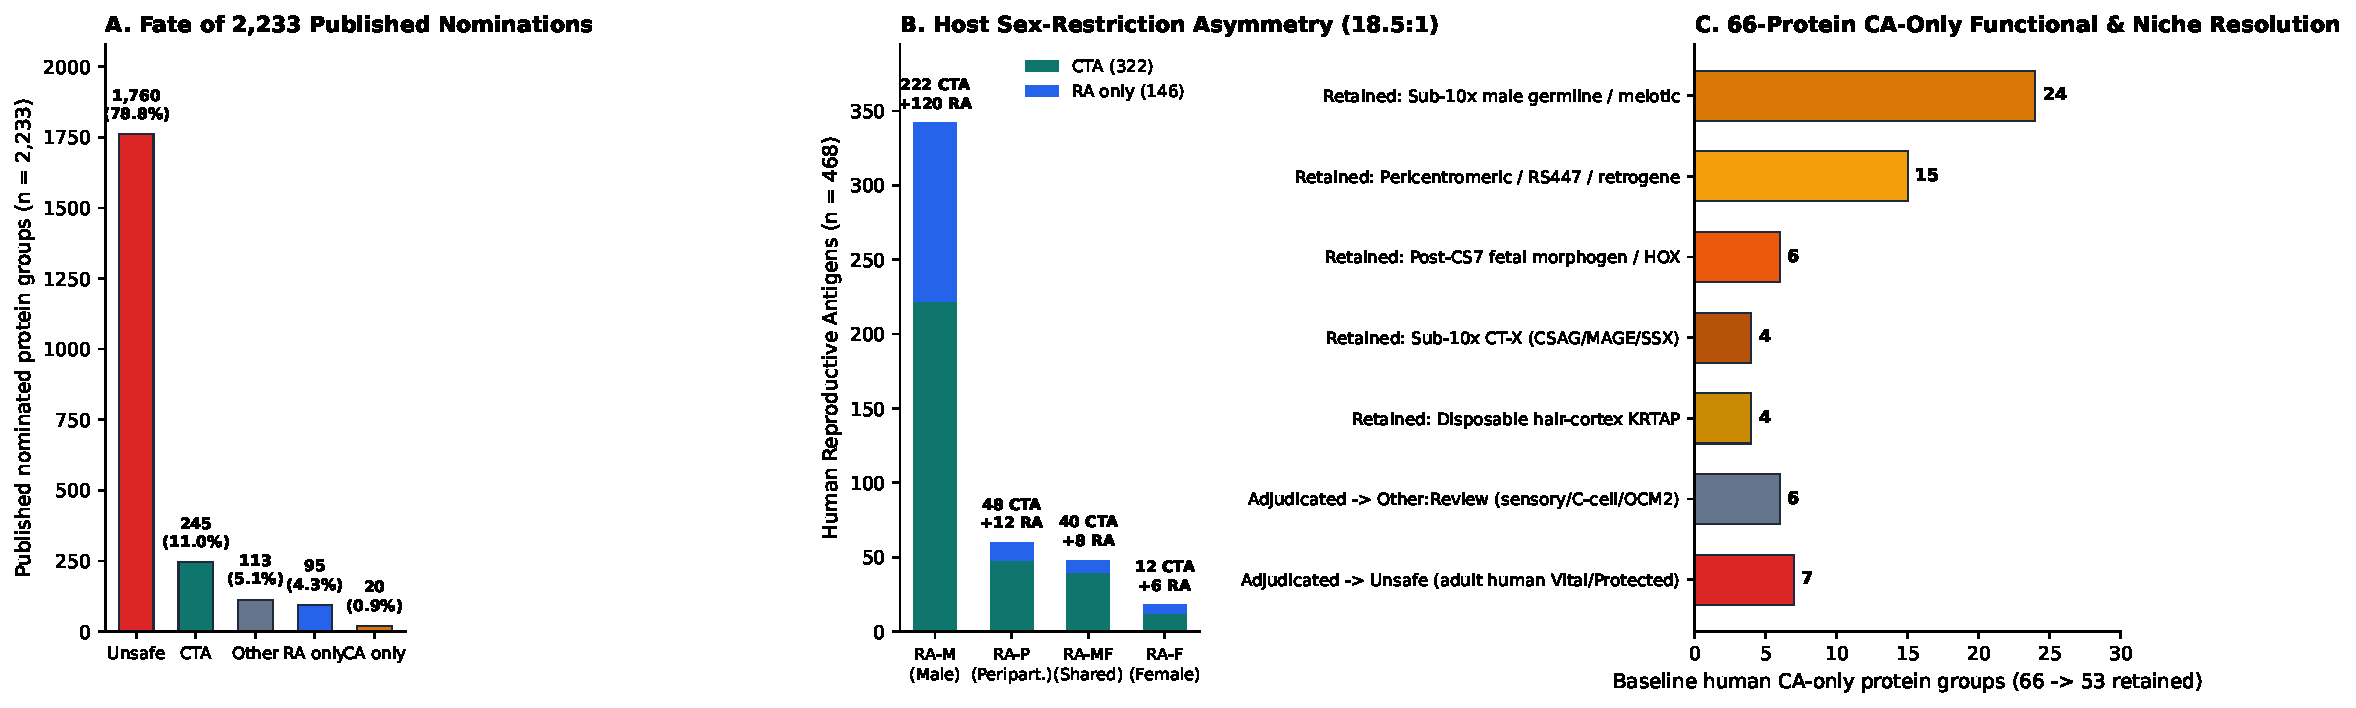
\includegraphics[width=\textwidth]{figures/fig3-human-deep-dive-and-ca-only-biology.pdf}
\caption{\textbf{Human literature reconciliation, sex-restriction asymmetry, and 66-protein \texttt{CA only} functional review.} \textbf{(A)} Disposition of 2,233 literature-nominated protein groups across 149 studies. \textbf{(B)} 4-way sex-restriction partition across 468 human RAs (322 CTAs). \textbf{(C)} Resolution of all 66 baseline \texttt{CA only} proteins into 7 \texttt{Unsafe}, 6 \texttt{Other:Review}, and 53 retained \texttt{CA only} across 5 biological classes.}
\label{fig:human}
\end{figure}

\textbf{Literature reconciliation and 18.5:1 sex asymmetry.} Of \textbf{2,233} published CTA/oncofetal nominations, \textbf{1,760 (78.8\%)} fail adult somatic gates (predominantly mitotic/centrosomal genes shared by spermatocytes, marrow, gut crypts, and activated lymphocytes), \textbf{113 (5.1\%)} enter \texttt{Other}, and \textbf{245} validate as \texttt{CTAs} alongside \textbf{77} newly identified expression-derived \texttt{CTAs} (Fig.~\ref{fig:human}A). Across the 322 \texttt{CTAs} (\textbf{311/322 = 96.6\%} with confirmed ectopic activation), \texttt{CTA-M} (222) outnumbers \texttt{CTA-F} (12) by \textbf{18.5:1}, complemented by \textbf{48} adult-absent peripartum \texttt{CTA-P} antigens (\textbf{270} female-safe vs.\ \textbf{60} male-safe \texttt{CTAs}; Fig.~\ref{fig:human}B). Auditing 159 female-lineage genes confirms this reflects continuous adult spermatogenesis behind the blood--testis barrier versus fetal completion of oogonial meiosis and sparse prophase-I oocytes ($<0.01\%$ of ovarian cortex, even with \texttt{GSE107746} isolated human oocytes), while true milk/placental proteins (\texttt{LALBA}, \texttt{CSN2}, \texttt{BTN1A1}, \texttt{PLAC1}, \texttt{ERVV-1/2}) populate \texttt{CTA-P}.

\begin{table}[htbp]
\centering
\scriptsize
\setlength{\tabcolsep}{3.5pt}
\caption{Primary-literature functional biology and micro-niche resolution of all 66 baseline human \texttt{CA only} (\texttt{CA $\setminus$ RA}) protein groups.}
\label{tab:caonly}
\begin{tabularx}{\textwidth}{p{3.1cm} r r p{5.4cm} X}
\toprule
\textbf{Disposition / Class} & \textbf{n} & \textbf{Med. Fold} & \textbf{Biological Mechanism \& Why R < 10x H0} & \textbf{Representative Proteins} \\
\midrule
Adjudicated -> Unsafe & 7 & 23.4x & Confirmed adult human Vital/Protected somatic micro-niche expression & GALP, BHLHE23, IL36B, ZACN, HES3, OCSTAMP, PROKR1 \\
Adjudicated -> Other:Review & 6 & 13.1x & Unscreened inner-ear/DRG sensory niche, diluted C-cell home, or 100\% 1-mm Unsafe paralog & SRMS, OCM2, CIB3, OTOP1, GFRA4, MRGPRG \\
Retained: Sub-10x male germline & 24 & 17.0x & Narrow spermatocyte/spermatid window or AZF/X copy diluted to 1x-9.6x in whole testis & PRDM9, RPS4Y2, RBMY1E (8.9x), ZNF705D (9.5x), LIPJ (9.6x), PKDREJ \\
Retained: Pericentromeric / RS447 & 15 & 20.1x & Hominoid macrosatellite arrays, cleavage ZGA duplications (<20-cell quorum), \& retrogenes & PRR20A-E, USP17L1/4/7, TRIM51G, TRIM64C, C1orf232, CCDC195 \\
Retained: Post-CS7 morphogen / HOX & 6 & 99.7x & Fetal tooth ameloblast scaffold \& post-gastrulation neural/limb homeobox TFs silent in adults & AMELX (30 pts), DBX1 (74 pts), HOXC12, HOXB1, HOXD12, EVX2 \\
Retained: Sub-10x CT-X paralogs & 4 & 29.7x & Canonical Xq28/Xp11/Xp21 cancer-germline loci whose bulk testis RNA sits below 10x N & CSAG3 (401 pts), CSAG2 (65 pts), SSX5 (8 pts), MAGEB17 \\
Retained: Disposable hair KRTAP & 4 & 12.8x & Anagen hair-shaft cortical matrix proteins cleared through Disposable <=32 TPM skin/hair screen & KRTAP20-3, KRTAP21-2, KRTAP21-3, KRTAP6-2 \\
\bottomrule
\end{tabularx}
\end{table}
\textbf{Functional resolution of all 66 \texttt{CA only} (\texttt{CA $\setminus$ RA}) proteins.} Auditing primary human literature, \texttt{HPA v25.1} single-cell \texttt{nCPM}, \texttt{\#735} mucosal/skeletal panels, and 1-mismatch \texttt{Unsafe} identity across all 66 pre-adjudication \texttt{CA only} proteins (Table~\ref{tab:caonly}, Fig.~\ref{fig:human}C) adjudicated \textbf{7} occult adult human \texttt{Vital}/\texttt{Protected} micro-niche proteins to \texttt{Unsafe}---\texttt{GALP} (adult human hypothalamic arcuate neuroendocrine neurons in \texttt{HYPOMAP} [16]), \texttt{BHLHE23} (adult human retinal rod/ON-cone bipolar neurons [17]), \texttt{IL36B} (epidermal/lingual keratinocytes [18]), \texttt{ZACN} (pancreas/brain/cardiac/olfactory $\text{Zn}^{2+}$ channel [19]), \texttt{HES3} (adult human pancreatic islet $\alpha/\beta$ cells [20]), \texttt{OCSTAMP} (multinucleated bone-resorbing osteoclasts [21]), and \texttt{PROKR1} (adrenal medulla/GI GPCR [22])---and \textbf{6} sensory/C-cell/paralog proteins (\texttt{SRMS}, \texttt{OCM2} with 0 safe $\ge 2$-mm 9-mers vs.\ \texttt{OCM}, inner-ear hair-cell \texttt{CIB3} [23,24] and \texttt{OTOP1} [25], thyroid parafollicular C-cell \texttt{GFRA4} [26,27], and DRG \texttt{MRGPRG}) to \texttt{Other:Review}. Every one of the \textbf{53} retained \texttt{CA only} proteins belongs to five transparent somatic-silent classes: sub-$10\times$ male germline/meiotic proteins (\textbf{24}: \texttt{PRDM9} [28], \texttt{RPS4Y2}, \texttt{RBMY1E} $8.9\times$, \texttt{ZNF705D} $9.5\times$, \texttt{LIPJ} $9.6\times$, \texttt{PKDREJ}), pericentromeric/\texttt{RS447} macrosatellites and 8-cell cleavage arrays (\textbf{15}: \texttt{PRR20A--E}, \texttt{USP17L1/4/7}, \texttt{C1orf232}, \texttt{CCDC195}), post-gastrulation fetal morphogens/\texttt{HOX} factors (\textbf{6}: \texttt{AMELX} [29], \texttt{DBX1} [30], \texttt{HOXC12/B1/D12}, \texttt{EVX2}), sub-$10\times$ \texttt{CT-X} paralogs (\textbf{4}: \texttt{CSAG3} in 401 patients, \texttt{CSAG2}, \texttt{SSX5}, \texttt{MAGEB17}), and \texttt{Disposable} hair-cortex \texttt{KRTAPs} (\textbf{4}).

\section{Empirical Calibration Against Clinical TCR-T and ImmTAC Trials}
\begin{figure}[htbp]
\centering
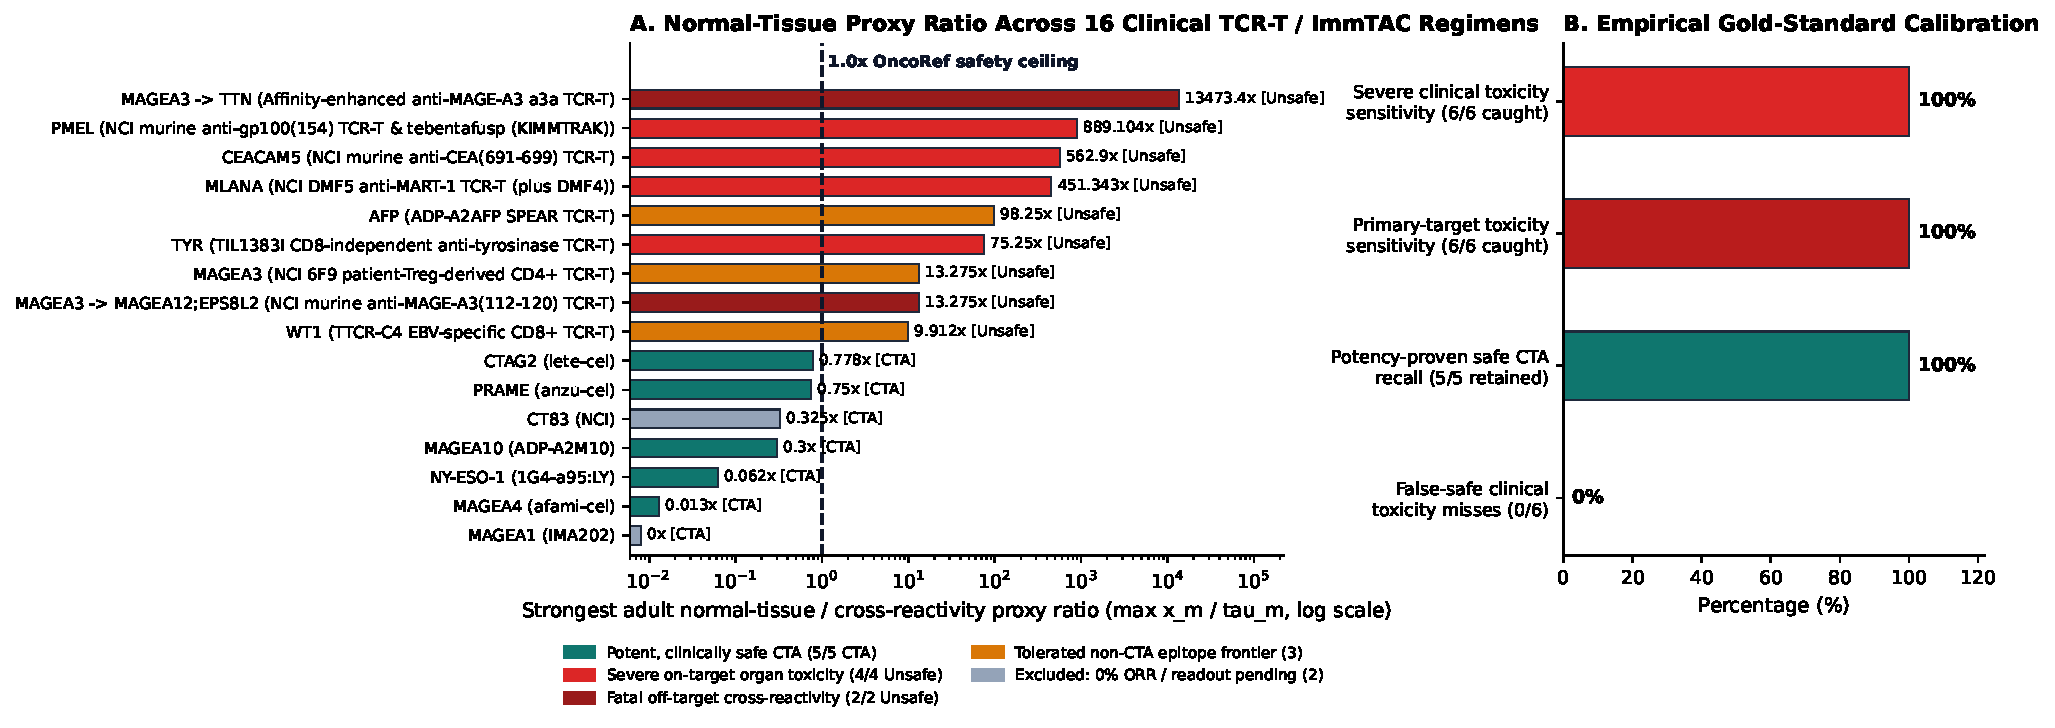
\includegraphics[width=\textwidth]{figures/fig4-clinical-tcr-gold-standard.pdf}
\caption{\textbf{Empirical calibration against 16 human clinical TCR-T and ImmTAC regimens.} \textbf{(A)} Maximum healthy adult normal or cross-reactive paralog ratio ($\max_m x_m / \tau_m$) vs.\ the $1.0\times$ OncoRef ceiling. \textbf{(B)} 100\% sensitivity (6/6) to clinical specificity toxicity and 100\% recall (5/5) on potent safe CTAs.}
\label{fig:tcr}
\end{figure}
\begin{table}[htbp]
\centering
\scriptsize
\setlength{\tabcolsep}{3.5pt}
\caption{Empirical calibration of OncoRef normal-tissue and paralog safety gates against 16 human clinical TCR-T and ImmTAC trial regimens.}
\label{tab:tcr}
\begin{tabularx}{\textwidth}{p{2.5cm} p{2.9cm} p{2.2cm} X p{2.5cm}}
\toprule
\textbf{Target} & \textbf{Product (HLA)} & \textbf{Potency} & \textbf{Observed Clinical Specificity Toxicity} & \textbf{OncoRef Call} \\
\midrule
NY-ESO-1 & 1G4-a95:LY / lete-cel (c259) (HLA-A*02:01;HLA-A*02:05;HLA-A*02:06) & n=38, 57.9\% ORR & Conditioning cytopenias and manageable CRS; zero attributed somatic solid-organ destruction (2 GBS cases across c259 program, 1 confounded day-161 cardiac arrest in MRCLS; separate TBI-1301 TCR had 1 steroid-responsive Gr3 lung infiltrate at 33\% ORR) & CTA (0.062x) \\
CTAG2 & lete-cel / NY-ESO-1-LAGE-1a c259 (HLA-A*02:01;HLA-A*02:05;HLA-A*02:06) & n=20, 30\% ORR & Conditioning cytopenias and CRS; zero pulmonary or urothelial toxicity despite first-pass IV lung perfusion & CTA (0.778x) \\
MAGEA4 & afami-cel / c1032 (TECELRA; FDA-approved) (HLA-A*02:01;HLA-A*02:02;HLA-A*02:03;HLA-A*02:06) & n=52, 36.5\% ORR & Conditioning cytopenias and CRS (71\% any-grade, 2\% Gr>=3); zero MAGE-A4-directed solid-organ injury (0 treatment-related deaths in SPEARHEAD-1; 1 MAGE-A4-negative marrow aplasia and 1 stroke in Phase 1) & CTA (0.013x) \\
PRAME & anzu-cel / IMA203 (plus brenetafusp ImmTAC) (HLA-A*02:01) & n=40, 52.5\% ORR & Conditioning cytopenias and mostly Gr1-2 CRS (1 reversible CRS-associated Gr4 transaminitis); zero clinical nephrotoxicity, adrenal insufficiency, or post-infusion treatment-related deaths & CTA (0.75x) \\
MAGEA10 & ADP-A2M10 / c796 SPEAR T-cells (HLA-A*02:01;HLA-A*02:06) & n=11, 9.1\% ORR & CRS (27\%; 1 resolved Gr4 CRS with Gr2 delirium) and 1 day-98 aplastic anemia death post-second lymphodepletion; zero MAGE-A10 solid-organ toxicity & CTA (0.3x) \\
CEACAM5 & NCI murine anti-CEA(691-699) TCR-T (HLA-A*02:01) & n=3, 33.3\% ORR & 3/3 (100\%) dose-limiting Grade 3 inflammatory pan-colitis from T-cell destruction of normal colonic mucosa (trial halted) & Unsafe (562.9x) \\
MLANA & NCI DMF5 anti-MART-1 TCR-T (plus DMF4) (HLA-A*02:01) & n=20, 30\% ORR & Severe on-target melanocyte destruction: erythematous skin rash/vitiligo (14/20, 70\%), anterior ocular uveitis (11/20, 55\%), and inner-ear sensorineural hearing loss/vestibular dysfunction (10/20, 50\%) & Unsafe (451.343x) \\
PMEL & NCI murine anti-gp100(154) TCR-T \& tebentafusp (KIMMTRAK) (HLA-A*02:01) & n=16, 18.8\% ORR & gp100 TCR-T: skin rash/vitiligo (15/16, 94\%), ocular uveitis (4/16, 25\%), hearing loss (5/16, 31\%); tebentafusp ImmTAC: >80\% rash/pruritus (\textasciitilde{}21\% Gr3) + vitiligo with minimal uveitis/ototoxicity & Unsafe (889.104x) \\
TYR & TIL1383I CD8-independent anti-tyrosinase TCR-T (HLA-A*02:01) & n=3, 33.3\% ORR & Progressive diffuse on-target vitiligo (cutaneous melanocyte destruction); ocular/uveal melanocyte risk flagged & Unsafe (75.25x) \\
MAGEA3 -> MAGEA12;EPS8L2 & NCI murine anti-MAGE-A3(112-120) TCR-T (HLA-A*02:01) & n=9, 55.6\% ORR & 3/9 severe neurotoxicity and 2/9 (22\%) FATAL necrotizing leukoencephalopathy / coma from cross-recognition of brain MAGEA12 (1-mm KMAELVHFL) and/or EPS8L2 (2-mm SAAELVHFL) & Unsafe (13.275x) \\
MAGEA3 -> TTN & Affinity-enhanced anti-MAGE-A3 a3a TCR-T (HLA-A*01:01) & n=2, lethal d4-5 & 2/2 (100\%) FATAL cardiogenic shock and myocardial T-cell necrosis within 4-5 days via 4-mismatch mimicry of cardiac titin (TTN ESDPIVAQY) & Unsafe (13473.4x) \\
MAGEA3 & NCI 6F9 patient-Treg-derived CD4+ TCR-T (HLA-DPB1*04:01) & n=17, 23.5\% ORR & Transient febrile CRS; zero neurotoxicity, cardiotoxicity, colitis, or treatment-related deaths & Unsafe (13.275x) \\
AFP & ADP-A2AFP SPEAR TCR-T (HLA-A*02:01) & n=21, 9.5\% ORR & Manageable CRS and cytopenias; no primary off-tumor autoimmune hepatitis or clinical nephrotoxicity & Unsafe (98.25x) \\
WT1 & TTCR-C4 EBV-specific CD8+ TCR-T (HLA-A*02:01) & n=12, 100\% RFS & Zero glomerular podocyte nephrotoxicity (no proteinuria/nephrotic syndrome) and zero mesothelial serositis (pleuritis/pericarditis) & Unsafe (9.912x) \\
MAGEA1 & IMA202 (HLA-A*02:01) & n=16, 0\% ORR & Cytopenias and Gr1-2 CRS without solid-organ toxicity; 0\% ORR precludes inferring in vivo cytolytic organ safety & CTA (0x) \\
CT83 & NCI / Rutgers anti-KK-LC-1 TCR-T (HLA-A*01:01) & Phase 1 pending & Pending peer-reviewed clinical readout & CTA (0.325x) \\
\bottomrule
\end{tabularx}
\end{table}
Across \textbf{16} curated endogenous-target clinical \texttt{TCR-T} and \texttt{ImmTAC} regimens (\textbf{14} potency-proven; Table~\ref{tab:tcr}, Fig.~\ref{fig:tcr}), OncoRef flags \textbf{6/6 (100\%, 0 false-safe misses)} severe specificity toxicities as \texttt{Unsafe} (\texttt{MAGEA3 $\rightarrow$ MAGEA12}, \texttt{MAGEA3 $\rightarrow$ TTN}, \texttt{CEACAM5}, \texttt{MLANA} \texttt{DMF5}/\texttt{DMF4}, \texttt{PMEL}, \texttt{TYR}) [6--9] while retaining \textbf{5/5 (100\%)} potency-proven safe \texttt{CTAs} (\texttt{MAGEA4} \emph{afami-cel}, \texttt{NY-ESO-1} and \texttt{CTAG2} \emph{lete-cel}, \texttt{PRAME} \texttt{IMA203}/\emph{brenetafusp}, \texttt{MAGEA10}) [1--5]. Three active non-CTA regimens (\texttt{WT1} \texttt{TCR-C4} immunoproteasome-differential \texttt{RMFPNAPYL} [31], \texttt{AFP}, and CD4 \texttt{HLA-DPB1*04:01} \texttt{MAGEA3} \texttt{KITE-718} [32]) define the epitope-processing frontier where whole-gene screening is intentionally conservative.

\section{Subcellular Localization \& Ectodomain Routing: CAR-T, ADC, and RLT}
\begin{figure}[htbp]
\centering
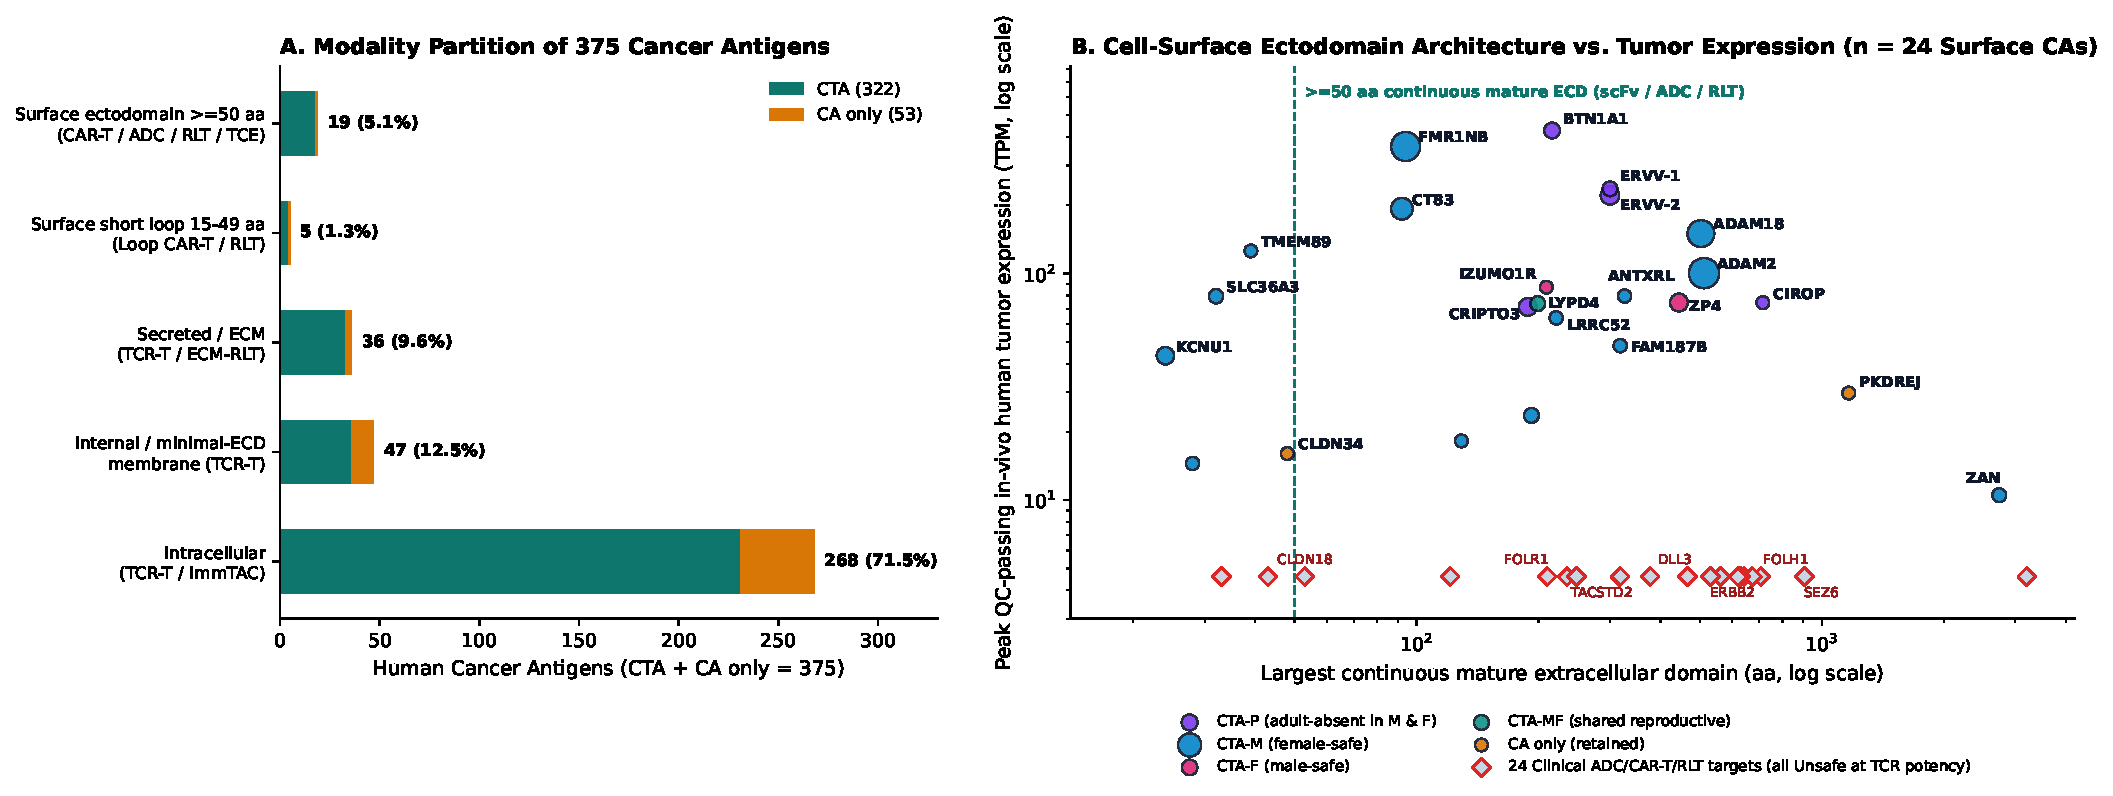
\includegraphics[width=\textwidth]{figures/fig5-surface-ectodomain-modality-routing.pdf}
\caption{\textbf{Subcellular localization and cell-surface ectodomain modality map.} \textbf{(A)} Partition of all 375 human Cancer Antigens (\texttt{322 CTA + 53 CA only}) across subcellular localization tiers. \textbf{(B)} Largest continuous mature extracellular domain (aa) vs.\ peak \emph{in vivo} tumor TPM across all 24 surface-exposed CAs alongside 24 clinical ADC/CAR-T/RLT benchmarks (all 24/24 \texttt{Unsafe} at TCR potency).}
\label{fig:surface}
\end{figure}
\begin{table}[htbp]
\centering
\scriptsize
\setlength{\tabcolsep}{3.5pt}
\caption{All 24 plasma-membrane extracellular-domain human Cancer Antigens (\texttt{CTA} $\cup$ \texttt{CA only}) actionable for CAR-T, ADC, TCE, or RLT modalities.}
\label{tab:surface}
\begin{tabularx}{\textwidth}{l l p{3.1cm} r p{2.3cm} p{2.3cm} r r}
\toprule
\textbf{Antigen} & \textbf{Class} & \textbf{Architecture} & \textbf{Max (Tot) ECD} & \textbf{ECD Span} & \textbf{Peak TPM} & \textbf{Pts} & \textbf{2mm 9m} \\
\midrule
ADAM2 & CTA-M & Single-pass Type I membrane & 512 (512) & 175-686 & 100.4 (BRCA) & 54 & 683 \\
FMR1NB & CTA-M & Multi-pass transmembrane (2 TM) & 94 (94) & 90-183 & 363.4 (MM) & 49 & 240 \\
ADAM18 & CTA-M & Single-pass Type I membrane & 503 (503) & 185-687 & 150.0 (LUSC) & 40 & 691 \\
CT83 & CTA-M & Single-pass Type II membrane & 92 (92) & 22-113 & 193.2 (CESC) & 22 & 102 \\
ERVV-2 & CTA-P & Multi-pass transmembrane (2 TM) & 300 (358) & 22-321;478-535 & 221.2 (KIRC) & 13 & 511 \\
ZP4 & CTA-F & Single-pass Type I membrane & 444 (444) & 19-462 & 74.4 (LUSC) & 11 & 518 \\
CRIPTO3 & CTA-P & Glycosylated surface coreceptor & 188 (188) & 1-188 & 71.2 (TGCT) & 11 & 0 \\
BTN1A1 & CTA-P & Single-pass Type I membrane & 216 (216) & 27-242 & 427.5 (BRCA) & 6 & 444 \\
ERVV-1 & CTA-P & Single-pass Type I membrane & 300 (300) & 22-321 & 236.4 (KIRP) & 4 & 457 \\
LYPD4 & CTA-MF & GPI-anchored ectodomain & 199 (199) & 27-225 & 73.7 (BRCA) & 4 & 234 \\
SPACA1 & CTA-M & Single-pass Type I membrane & 192 (192) & 30-221 & 23.6 (KIRC) & 4 & 280 \\
ZAN & CTA-M & Single-pass Type I membrane & 2740 (2740) & 18-2757 & 10.5 (TGCT) & 2 & 2529 \\
ANTXRL & CTA-M & Single-pass Type I membrane & 326 (326) & 28-353 & 79.5 (OV) & 1 & 572 \\
LRRC52 & CTA-M & Single-pass Type I membrane & 221 (221) & 24-244 & 63.7 (SKCM) & 1 & 294 \\
FAM187B & CTA-M & Single-pass Type I membrane & 318 (318) & 18-335 & 48.1 (BRCA) & 1 & 348 \\
IZUMO1R & CTA-F & GPI-anchored ectodomain & 209 (209) & 20-228 & 87.0 (MENINGIOMA) & 0 & 208 \\
CIROP & CTA-P & Single-pass Type I membrane & 715 (715) & 21-735 & 74.4 (MENINGIOMA) & 0 & 708 \\
PKDREJ & CA only & Multi-pass transmembrane (11 TM) & 1165 (1487) & 20-1184;1411-1427;1598-1607;1730-1966;2018-2042;2113-2145 & 29.7 (NEC\_MERKEL) & 0 & 2189 \\
TMEM95 & CTA-M & Single-pass Type I membrane & 129 (129) & 17-145 & 18.3 (NEC\_MERKEL) & 0 & 161 \\
TMEM89 & CTA-M & Single-pass Type I membrane & 39 (39) & 25-63 & 125.8 (NEC\_MERKEL) & 0 & 141 \\
SLC36A3 & CTA-M & Multi-pass transmembrane (11 TM) & 32 (112) & 68-71;159-185;232-252;306-337;389-392;447-470 & 79.4 (B\_ALL) & 3 & 351 \\
KCNU1 & CTA-M & Multi-pass transmembrane (7 TM) & 24 (65) & 1-24;123-138;185-188;248-259;283-291 & 43.4 (LIHC) & 10 & 1077 \\
CLDN34 & CA only & Multi-pass transmembrane (4 TM) & 48 (79) & 33-80;147-177 & 16.1 (NEC\_MERKEL) & 0 & 205 \\
CXorf66 & CTA-M & Single-pass Type I membrane & 28 (28) & 20-47 & 14.5 (BRCA) & 1 & 345 \\
\bottomrule
\end{tabularx}
\end{table}
Mapping SHA-256-pinned UniProtKB topological domains, cleaved signal/propeptide spans, transmembrane helices, and \texttt{GPI}-anchors onto Ensembl 115 sequences across all \textbf{375} human \texttt{CAs} reveals that \textbf{315 (84.0\%)} are intracellular (268 nuclear/cytoplasmic/cytoskeletal including \texttt{PRAME}, \texttt{NY-ESO-1}, \texttt{MAGEA4}, \texttt{DUX4}, and fibrous-sheath \texttt{AKAP4}; 47 internal/minimal-ECD membrane) and \textbf{36 (9.6\%)} are secreted (\texttt{CSN2}, \texttt{LALBA}, \texttt{PLAC1}, \texttt{AMELX}), making \texttt{pMHC}-directed \texttt{TCR-T}/\texttt{ImmTAC} obligatory for $>84\%$ of somatic-silent antigens (Fig.~\ref{fig:surface}A). Conversely, \textbf{24/24 (100\%)} of conventional clinical \texttt{ADC}/\texttt{CAR-T}/\texttt{RLT} benchmarks (\texttt{HER2}, \texttt{TROP2}, \texttt{FR$\alpha$}, \texttt{PSMA}, \texttt{SSTR2}, \texttt{DLL3}, \texttt{CLDN18.2}, \texttt{CLDN6}, \texttt{MSLN}, \texttt{GPC3}, \texttt{ROR1}, \texttt{STEAP1}, \texttt{SEZ6}) are \texttt{Unsafe} at \texttt{TCR} potency because they rely on surface receptor-density windows or luminal polarization.

Strikingly, \textbf{24 human Cancer Antigens (22 \texttt{CTAs} + 2 \texttt{CA only})} combine \textbf{TCR-grade adult somatic silence} with \textbf{plasma-membrane extracellular exposure} (Table~\ref{tab:surface}, Fig.~\ref{fig:surface}B): \textbf{19} carry substantial $\ge 50\text{ aa}$ continuous mature ectodomains directly suited for \texttt{CAR-T}, \texttt{ADC}, \texttt{TCE}, and \texttt{RLT}---led by adult-absent peripartum \texttt{CTA-P} targets \textbf{\texttt{BTN1A1}} (216 aa IgV--IgC checkpoint ectodomain, 427.5 TPM [33]), retroviral envelopes \textbf{\texttt{ERVV-1}} and \textbf{\texttt{ERVV-2}} (300 aa \texttt{SU} ectodomains, 236--221 TPM in \texttt{KIRP}/\texttt{KIRC}), \textbf{\texttt{CIROP}} (715 aa), and \textbf{\texttt{CRIPTO3}} (188 aa EGF-CFC coreceptor, 11 \texttt{TGCT} patients); high-prevalence \texttt{CTA-M} metalloproteinase-like \textbf{\texttt{ADAM2}} (512 aa mature ECD, 54 patients) and \textbf{\texttt{ADAM18}} (503 aa, 40 patients), \textbf{\texttt{FMR1NB}} (94 aa loop, 49 patients), and Type II \textbf{\texttt{CT83}} (92 aa ECD, 22 patients [34]); \texttt{CTA-F} \textbf{\texttt{ZP4}} (444 aa, 11 patients) and \texttt{GPI}-anchored folate-receptor paralog \textbf{\texttt{IZUMO1R}} (209 aa, structurally homologous to \texttt{FOLR1}); \texttt{CTA-MF} \textbf{\texttt{LYPD4}} (199 aa \texttt{GPI}-anchored Ly6/uPAR fold); and \texttt{CA only} \textbf{\texttt{PKDREJ}} (1,165 aa REJ/GPS ECD)---plus \textbf{5} constrained 24--48 aa loop targets including 4-TM claudin \textbf{\texttt{CLDN34}} (48 aa ECL1, matching \texttt{CLDN18.2}/\texttt{CLDN6} topology).

\section{Limitations and Data \& Code Availability}
Peak bulk tumor \texttt{TPM} requires spatial \texttt{IHC}/\texttt{RNAscope} clonality validation; \texttt{TCR-T} candidates require immunopeptidomic confirmation; fetal mid-gestation organogenesis remains fail-closed (\texttt{pregnant=True}); and canonical surface topologies require tumor isoform/shedding verification. All data, SHA-256 receipts, and deterministic build scripts (\texttt{oncoref==1.55+}) are openly available under Apache 2.0 at \url{https://github.com/pirl-unc/oncoref}.

\small
\begin{thebibliography}{34}\setlength{\itemsep}{1pt}
\bibitem{r1} D'Angelo SP et al. NY-ESO-1 c259T cells in synovial sarcoma. \emph{Cancer Discov.} 2018;8:944--957 (PMID:29891538).
\bibitem{r2} D'Angelo SP et al. Afamitresgene autoleucel (SPEARHEAD-1). \emph{Lancet.} 2024;403:1460--1471 (PMID:38552654).
\bibitem{r3} Pollack SM et al. Letetresgene autoleucel in MRCLS. \emph{J Clin Oncol.} 2025 (PMC12084024).
\bibitem{r4} Wermke M et al. Autologous PRAME TCR-T (IMA203) Phase 1. \emph{Nat Med.} 2025 (PMID:40200105).
\bibitem{r5} Hamid O et al. Brenetafusp (IMC-F106C) PRAME ImmTAC in melanoma. \emph{J Clin Oncol / ESMO.} 2024.
\bibitem{r6} Morgan RA et al. Neurological toxicity after anti-MAGE-A3 TCR therapy. \emph{J Immunother.} 2013;36:133--151 (PMID:23377668).
\bibitem{r7} Linette GP et al. Titin cross-reactivity of MAGE-A3 TCR T cells. \emph{Blood.} 2013;122:863--871 (PMID:23770775).
\bibitem{r8} Parkhurst MR et al. CEA TCR T cells induce severe transient colitis. \emph{Mol Ther.} 2011;19:620--626 (PMID:21157437).
\bibitem{r9} Johnson LA et al. MART-1 and gp100 TCR therapy targets normal melanocytes. \emph{Blood.} 2009;114:535--546 (PMID:19451487).
\bibitem{r10} Almeida LG et al. CTdatabase. \emph{Nucleic Acids Res.} 2009;37:D816--D819 (PMID:18838390).
\bibitem{r11} Wang C et al. Systematic identification of cancer-testis genes in 19 cancer types. \emph{Nat Commun.} 2016;7:10499 (PMID:26813868).
\bibitem{r12} da Silva VL et al. Pan-cancer identification of cancer/testis genes. \emph{Oncotarget.} 2017;8:92966--92977 (PMID:29190970).
\bibitem{r13} Bruggeman JW et al. Germ cell-specific genes expressed in human cancers. \emph{Oncotarget.} 2018;9:29795--29812 (PMID:30042815).
\bibitem{r14} Carter JA et al. Pan-cancer analysis of cancer-testis antigens. \emph{J Immunother Cancer.} 2023 (PMID:37369392).
\bibitem{r15} Van den Eynde B et al. Murine mastocytoma antigen P1A (\texttt{Trap1a}). \emph{J Exp Med.} 1991;173:1373--1384; Sarma S et al. \emph{J Exp Med.} 1999;189:811--820.
\bibitem{r16} Tadross JA et al. Spatio-cellular map of the human hypothalamus (\texttt{HYPOMAP}). \emph{Nature.} 2025;638:1049--1059 (PMID:39910309).
\bibitem{r17} Cowan CS et al. Cell types of the human retina at single-cell resolution. \emph{Cell.} 2020;182:1623--1640 (PMID:32946783).
\bibitem{r18} Johnston A et al. IL-36 cytokines in human keratinocytes. \emph{J Immunol.} 2011;186:2613--2622 (PMID:21242515).
\bibitem{r19} Davies PA et al. Zinc-activated channel (\texttt{ZACN}) in human pancreas and brain. \emph{J Biol Chem.} 2003;278:712--717 (PMID:12381728).
\bibitem{r20} Masjkur J et al. Hes3 in adult human pancreatic islets. \emph{J Biol Chem.} 2014;289:35503--35516 (PMID:25371201).
\bibitem{r21} Khan UA et al. OC-STAMP in human osteoclast multinucleation. \emph{J Cell Biochem.} 2013;114:1772--1781 (PMID:23444125).
\bibitem{r22} Lin DC et al. Prokineticin receptor 1 (\texttt{PROKR1}). \emph{J Biol Chem.} 2002;277:19276--19280 (PMID:11886876).
\bibitem{r23} van der Valk WH et al. Single-cell atlas of human cochlea and vestibular organs. \emph{Cell Rep.} 2023;42:112623 (PMID:37289589).
\bibitem{r24} Liang X et al. CIB2 and CIB3 hair-cell MET channel subunits. \emph{EMBO J.} 2021;40:e107279 (PMID:34487363).
\bibitem{r25} Tu YH et al. Proton-selective ion channel OTOP1 in sour taste cells. \emph{Science.} 2018;359:1047--1050 (PMID:29371428).
\bibitem{r26} Lindahl M et al. Human GFR$\alpha$4 in thyroid parafollicular C-cells. \emph{J Biol Chem.} 2001;276:9344--9351 (PMID:11116144).
\bibitem{r27} Bhoj VG et al. GFR$\alpha$4 CAR-T in medullary thyroid cancer. \emph{Mol Ther Oncolytics.} 2021;20:387--398 (PMID:33632929).
\bibitem{r28} Baudat F et al. PRDM9 determines meiotic recombination hotspots. \emph{Science.} 2010;327:836--840 (PMID:20044539).
\bibitem{r29} Salido EC et al. Human amelogenin (\texttt{AMELX}). \emph{Am J Hum Genet.} 1992;50:303--316; Apps JR et al. \emph{J Pathol.} 2018;244:458--469.
\bibitem{r30} Pierani A et al. Progenitor homeodomain protein Dbx1. \emph{Neuron.} 2001;29:367--384 (PMID:11239428).
\bibitem{r31} Chapuis AG et al. WT1 TCR-C4 therapy post-transplant in AML. \emph{Nat Med.} 2019;25:1064--1072 (PMID:31235963).
\bibitem{r32} Lu YC et al. MHC class II-restricted MAGE-A3 TCR (KITE-718). \emph{J Clin Oncol.} 2017;35:3322--3329 (PMID:28809608).
\bibitem{r33} Seo M et al. BTN1A1 immune checkpoint (hSTC810). \emph{J Immunother Cancer.} 2024;12:e008303 (PMID:38490683).
\bibitem{r34} Marcinkowski B et al. TCR-T targeting CT83 (KK-LC-1). \emph{J Immunother Cancer.} 2019;7:229 (PMID:31462308).
\end{thebibliography}
\end{document}
